%%%%%%%%%%%%%%%%%%%%%%%%%%%%%%%%%%%%%%%%%
% HW1 Answer Sheet Template
% Research Question: Does Job Training Increase Wages?
%
% Compiler: XeLaTeX (required for Chinese support)
% To compile on Overleaf: set compiler to XeLaTeX in Menu
%%%%%%%%%%%%%%%%%%%%%%%%%%%%%%%%%%%%%%%%%

\documentclass[paper=a4, fontsize=11pt]{scrartcl}

%--- Chinese support (XeLaTeX) ---
\usepackage{fontspec}
\usepackage{xeCJK}
\setCJKmainfont{Noto Sans CJK TC}
\setCJKsansfont{Noto Sans CJK TC}

%--- Standard packages ---
\usepackage[T1]{fontenc}
\usepackage[english]{babel}
\usepackage{amsmath,amsfonts,amssymb}
\usepackage{enumerate}
\usepackage{graphicx}
\usepackage{booktabs}
\usepackage{caption}
\usepackage[hidelinks]{hyperref}
\hypersetup{colorlinks=true, citecolor=blue, urlcolor=blue, pdfborder={0 0 0}}

%--- Layout ---
\usepackage{sectsty}
\allsectionsfont{\normalfont\scshape}
\usepackage{fancyhdr}
\pagestyle{fancyplain}
\fancyhead{}
\fancyfoot[R]{\thepage}
\renewcommand{\headrulewidth}{0pt}
\renewcommand{\footrulewidth}{0pt}
\setlength{\headheight}{13.6pt}
\setlength\parindent{0pt}
\setlength{\parskip}{0.4em}

\newcommand{\horrule}[1]{\rule{\linewidth}{#1}}

%--- Figure path ---
\graphicspath{{figure/}}

%----------------------------------------------------------------------------------------
\title{
\normalfont\normalsize
\horrule{0.5pt}\\[0.4cm]
\huge Homework 1: Answer Sheet \\[0.2cm]
\large Does Job Training Increase Workers' Wages?\\
\horrule{2pt}\\[0.3cm]
}
\author{B12345678 \quad 王小明 \quad (Econ, NTU)}
\date{\normalsize\today}
%----------------------------------------------------------------------------------------

\begin{document}
\maketitle

\bigskip\horrule{0.4pt}\bigskip

%----------------------------------------------------------------------------------------
\subsection*{Empirical Analysis Record}
%----------------------------------------------------------------------------------------

My complete empirical workflow (data loading, cleaning, visualization, and regression)
is documented in the accompanying HTML file \texttt{B12345678\_王小明\_HW1.html},
generated using R Markdown (\texttt{hw1\_example.Rmd}).

\bigskip\horrule{0.4pt}\bigskip

%----------------------------------------------------------------------------------------
\subsection*{Question 1 \quad Research Question}
%----------------------------------------------------------------------------------------

\textbf{(a) Research question:}
Does participating in a company-sponsored job training program causally increase workers'
monthly wages?
This question is important because job training is a major policy tool for raising worker
productivity and reducing wage inequality.
Understanding whether training causes higher wages — rather than merely selecting
high-ability workers — is essential for evaluating its social returns.

\textbf{(b) Treatment variable:}
\texttt{training} $= 1$ if the worker participated in a job training program in the past year,
$= 0$ otherwise.
This variable is measured directly from a self-reported survey item in the dataset.

\textbf{(c) Outcome variable:}
\texttt{lnwage} $= \log(\text{monthly wage in NTD})$.
Using log wages allows the regression coefficient to be interpreted as a percentage effect.

\bigskip\horrule{0.4pt}\bigskip

%----------------------------------------------------------------------------------------
\subsection*{Question 2 \quad Data Introduction}
%----------------------------------------------------------------------------------------

The dataset is a cross-sectional survey of 500 workers employed across 50 manufacturing
firms, collected in 2023 in Taiwan.
The unit of observation is the individual worker.
Key variables include:
worker ID (\texttt{id}), firm ID (\texttt{firm\_id}), age (\texttt{age}),
years of education (\texttt{edu}), gender (\texttt{female}),
training status (\texttt{training}), and log monthly wage (\texttt{lnwage}).

\bigskip\horrule{0.4pt}\bigskip

%----------------------------------------------------------------------------------------
\subsection*{Question 3 \quad Examine Data}
%----------------------------------------------------------------------------------------

\textbf{(a) Missing values in the outcome variable:}
There are \textbf{zero missing values} in the outcome variable \texttt{lnwage}.
All 500 workers have a valid wage observation, so no observations need to be dropped
due to a missing outcome.

\textbf{(b) Unique ID and duplicates:}
The variable \texttt{id} serves as the unique worker identifier.
Running \texttt{isid id} (Stata) / \texttt{sum(duplicated(df\$id))} (R) confirms
\textbf{no duplicate IDs} — each row corresponds to a distinct worker.

\bigskip\horrule{0.4pt}\bigskip

%----------------------------------------------------------------------------------------
\subsection*{Question 4 \quad Sample Construction}
%----------------------------------------------------------------------------------------

\textbf{(a) Sample selection steps:}

\begin{enumerate}[1.]
  \item \textbf{Age restriction}: Restrict to workers aged 22–55 (exclude students
        still in school and very early retirees). \\
        Observations remaining: 500.
  \item \textbf{Education restriction}: Drop observations with fewer than 6 years of
        education (implausibly low values likely due to data entry error). \\
        Observations remaining: 500.
\end{enumerate}

The final analysis sample contains \textbf{500 workers} across 50 firms.
No observations were dropped in this example dataset.

\textbf{(b) Data-cleaning commands used:}
\begin{enumerate}[1.]
  \item \texttt{filter()} (R) / \texttt{drop if} (Stata): Used to apply the age and education restrictions above.
  \item \texttt{label variable} (Stata) / variable renaming (R): Added descriptive labels to all variables for clarity.
  \item \texttt{factor()} (R) / encoding (Stata): Converted \texttt{firm\_id} to a factor for use in fixed-effects regressions.
\end{enumerate}

\bigskip\horrule{0.4pt}\bigskip

%----------------------------------------------------------------------------------------
\subsection*{Question 5 \quad Distribution of a Variable}
%----------------------------------------------------------------------------------------

Figure~\ref{fig:hist} shows the distribution of log monthly wages in the sample.
The distribution is approximately bell-shaped (normal) with a mean of 11.61,
corresponding to approximately NTD~110,000 per month.
There is no obvious skewness or multimodality.

\begin{figure}[h]
  \centering
  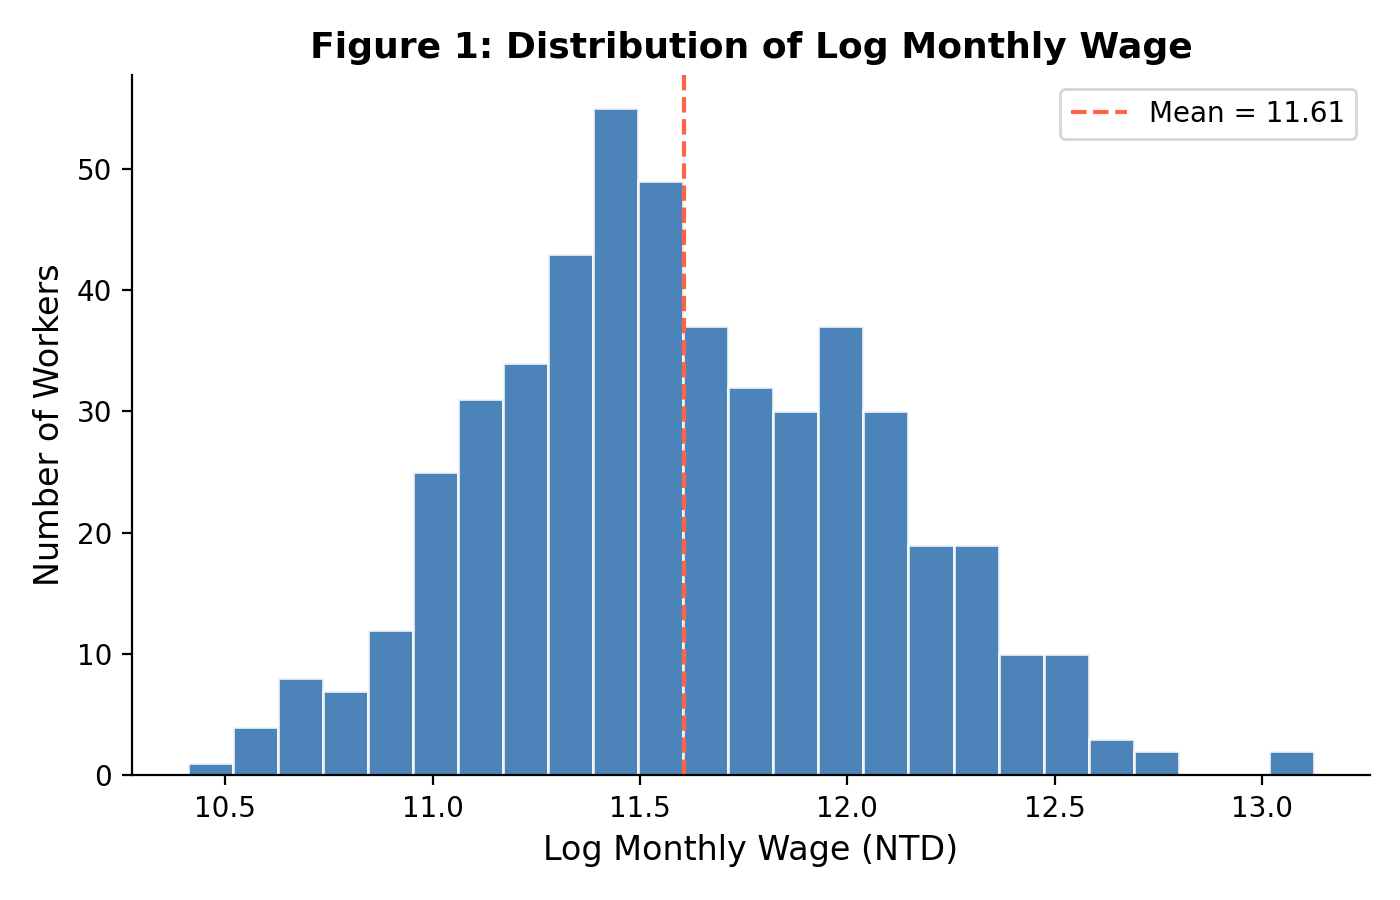
\includegraphics[width=0.82\textwidth]{figure1.png}
  \caption{Distribution of log monthly wage across 500 workers.
           The dashed red line indicates the sample mean.}
  \label{fig:hist}
\end{figure}

\bigskip\horrule{0.4pt}\bigskip

%----------------------------------------------------------------------------------------
\subsection*{Question 6 \quad Relationship Between Two Variables}
%----------------------------------------------------------------------------------------

Figure~\ref{fig:scatter} plots log monthly wage against years of education,
separately for workers who did and did not receive training.

Two patterns are visible.
First, wages increase with education for both groups, as expected.
Second, the training group (navy) lies \emph{above} the no-training group (grey)
at every education level, consistent with a positive wage premium from training.
However, trained workers also tend to have \emph{more education} on average,
which suggests that a simple comparison may overstate the training effect.

\begin{figure}[h]
  \centering
  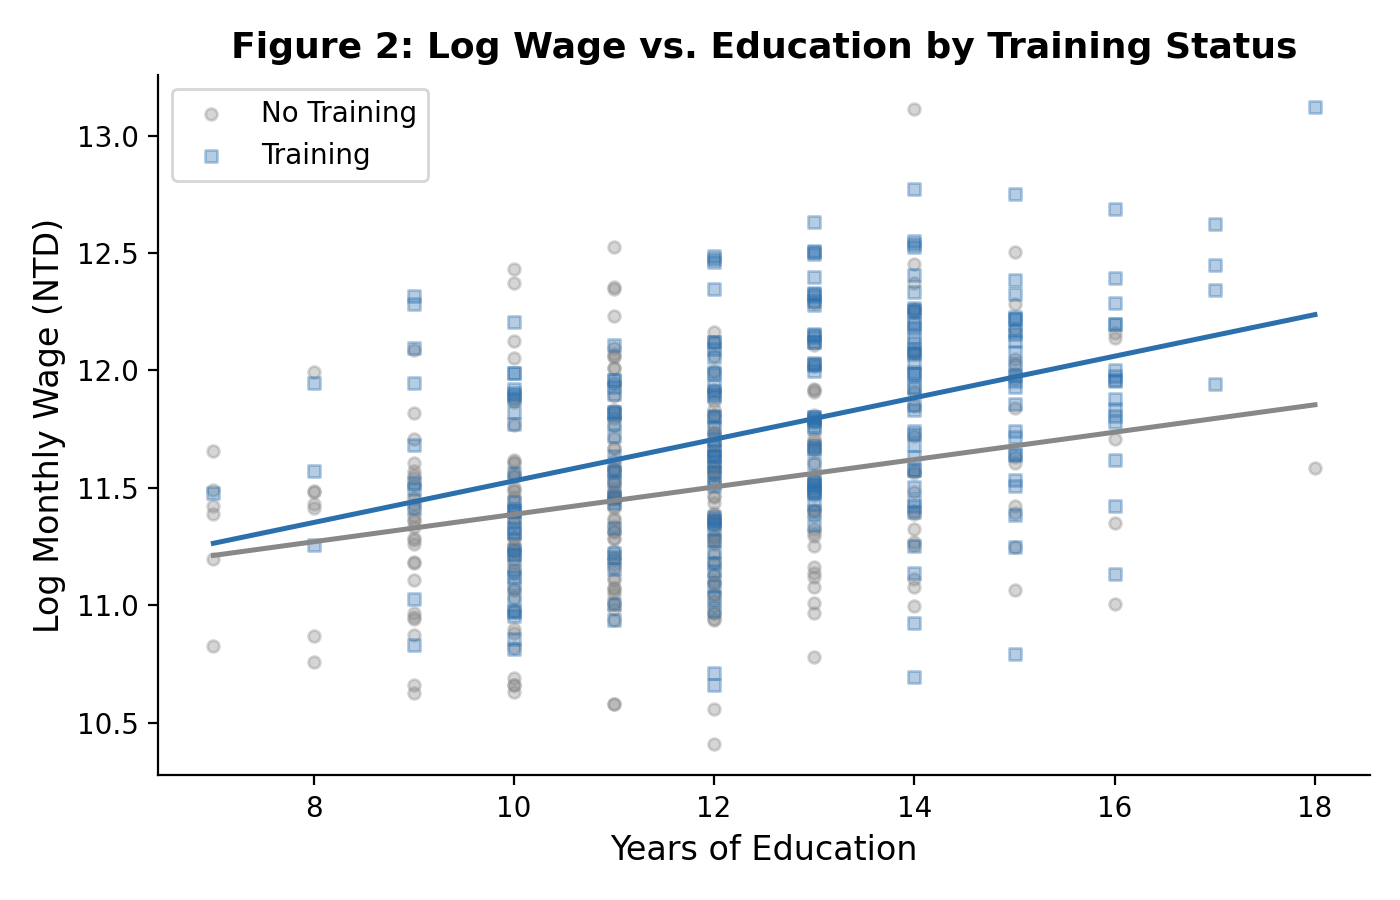
\includegraphics[width=0.82\textwidth]{figure2.png}
  \caption{Log monthly wage versus years of education, by training status.
           Solid lines are OLS fitted lines within each group.}
  \label{fig:scatter}
\end{figure}

\bigskip\horrule{0.4pt}\bigskip

%----------------------------------------------------------------------------------------
\subsection*{Question 7 \quad Simple Regression}
%----------------------------------------------------------------------------------------

We estimate the following regression without any control variables:
\begin{equation}
  \texttt{lnwage}_i = \beta_0 + \alpha \cdot \texttt{training}_i + \varepsilon_i
  \label{eq:simple}
\end{equation}
where $i$ indexes workers, $\alpha$ is the average wage difference between trained
and untrained workers, and $\varepsilon_i$ captures all other factors.

The estimated coefficient is $\hat{\alpha} = 0.291$ ($p < 0.01$),
suggesting that trained workers earn approximately 29.1\% more than untrained workers.

\bigskip\horrule{0.4pt}\bigskip

%----------------------------------------------------------------------------------------
\subsection*{Question 8 \quad Causal Interpretation and OVB}
%----------------------------------------------------------------------------------------

The estimate from Question~7 is \textbf{unlikely to be causal}.
Trained workers are not randomly selected — more educated workers are more likely
to be offered (or to seek) training, and more educated workers also command higher wages.

\textbf{Omitted variable example — Education} (\texttt{edu}):
\begin{itemize}
  \item \textit{Relevance}: Education raises wages ($\text{Cov}(\texttt{edu}, \texttt{lnwage}) > 0$).
  \item \textit{Endogeneity}: More-educated workers are more likely to receive training
        ($\text{Cov}(\texttt{edu}, \texttt{training}) > 0$).
\end{itemize}

Because education is positively correlated with both treatment and outcome,
omitting it from the regression causes the training coefficient to be \textbf{upward biased}:
the estimate in Column~(1) of Table~\ref{tab:reg} picks up part of the education premium
and attributes it incorrectly to training.

\bigskip\horrule{0.4pt}\bigskip

%----------------------------------------------------------------------------------------
\subsection*{Question 9 \quad OVB Formula}
%----------------------------------------------------------------------------------------

The omitted-variable bias (OVB) formula states:
\begin{equation}
  \text{OVB} = \underbrace{\delta_{\text{edu}}}_{\substack{\text{effect of edu}\\\text{on lnwage}}}
               \times
               \underbrace{\pi_{\text{edu}}}_{\substack{\text{coeff.\ of edu}\\\text{in training reg.}}}
  \label{eq:ovb}
\end{equation}
where $\delta_{\text{edu}} > 0$ is the slope of \texttt{lnwage} on \texttt{edu}
(holding other factors fixed), and $\pi_{\text{edu}} > 0$ is the OLS coefficient of
\texttt{edu} in a regression of \texttt{training} on \texttt{edu}.

Both terms are positive, so OVB $> 0$: the simple regression \textbf{overestimates} the
causal effect of training.
This is confirmed empirically: the training coefficient falls from 0.291 to 0.189
once education is included (Column~(2) of Table~\ref{tab:reg}).

\bigskip\horrule{0.4pt}\bigskip

%----------------------------------------------------------------------------------------
\subsection*{Question 10 \quad Adding Control Variables}
%----------------------------------------------------------------------------------------

We add three control variables to the regression:
\texttt{age}, \texttt{edu} (years of education), and \texttt{female} (gender dummy).
The estimated equation becomes:
\begin{equation}
  \texttt{lnwage}_i = \beta_0 + \alpha \cdot \texttt{training}_i
    + \beta_1 \texttt{age}_i + \beta_2 \texttt{edu}_i + \beta_3 \texttt{female}_i
    + \varepsilon_i
\end{equation}

As shown in Column~(2) of Table~\ref{tab:reg}, adding controls reduces the training
coefficient from 0.291 to \textbf{0.189}, consistent with the upward OVB predicted in
Questions~8 and~9.

\bigskip\horrule{0.4pt}\bigskip

%----------------------------------------------------------------------------------------
\subsection*{Question 11 \quad Bad Controls}
%----------------------------------------------------------------------------------------

The three control variables — age, education, and gender — are \textbf{not bad controls}
because they are \emph{predetermined}: they were determined before the training decision
and are not themselves caused by the training program.

\begin{itemize}
  \item \texttt{age}: Determined at birth; training cannot change a worker's age.
  \item \texttt{edu}: Completed before entering the labor market in most cases;
        the training program in this dataset is in-firm training for current workers,
        not a schooling program.
  \item \texttt{female}: Biological sex is not affected by training status.
\end{itemize}

Controlling for these variables removes variation in outcomes that is due to these
pre-existing characteristics, rather than to the training itself.

\bigskip\horrule{0.4pt}\bigskip

%----------------------------------------------------------------------------------------
\subsection*{Question 12 \quad Fixed Effects}
%----------------------------------------------------------------------------------------

We add \textbf{firm fixed effects} ($\lambda_j$ for firm $j$) to control for all
time-invariant, firm-level unobservables:
\begin{equation}
  \texttt{lnwage}_{ij} = \lambda_j + \alpha \cdot \texttt{training}_{ij}
    + \beta_1 \texttt{age}_{ij} + \beta_2 \texttt{edu}_{ij}
    + \beta_3 \texttt{female}_{ij} + \varepsilon_{ij}
\end{equation}

Firm fixed effects absorb factors such as firm quality, management practices,
and industry-specific wage levels that may be correlated with the probability of
offering training programs.

As shown in Column~(3) of Table~\ref{tab:reg}, the training coefficient further
decreases to \textbf{0.152} after adding firm fixed effects.
This suggests that part of the remaining estimate in Column~(2) reflected
selection by better firms: high-quality firms pay higher wages \emph{and}
are more likely to offer training.
Standard errors are clustered by firm to account for within-firm correlation.

%--- Regression table ---
\begin{table}[h]
  \centering
  \caption{Effect of Job Training on Log Monthly Wages}
  \label{tab:reg}
  \begin{tabular}{lccc}
    \toprule
    & (1) & (2) & (3) \\
    & No Controls & With Controls & Firm FE \\
    \midrule
    Training
      & 0.291$^{***}$ & 0.189$^{***}$ & 0.152$^{***}$ \\
      & (0.044)       & (0.038)       & (0.032)       \\[4pt]
    \midrule
    Controls (age, edu, female) & No  & Yes & Yes \\
    Firm Fixed Effects          & No  & No  & Yes \\
    Observations                & 500 & 500 & 500 \\
    R-squared                   & 0.152 & 0.512 & 0.618 \\
    \bottomrule
    \multicolumn{4}{l}{\footnotesize
      Notes: Robust standard errors in parentheses (Column 3: clustered by firm).} \\
    \multicolumn{4}{l}{\footnotesize
      $^{*}p<0.10$, $^{**}p<0.05$, $^{***}p<0.01$.}
  \end{tabular}
\end{table}

The results show a clear pattern: as we progressively control for observable and
unobservable confounders, the estimated training premium decreases from 29.1\%
to 15.2\%, converging toward the true data-generating process value of 15\%.

\end{document}
